\section{Parcelamiento del hemisferio izquierdo}

Luego de dividir el \'area de Broca parcelamos todo el hemisferio
izquierdo del sujeto. Nuevamente situamos semillas a $3mm$ de la corteza
siguiendo la secci\'on \ref{sec:semillas} y generamos tractogramas
utilizando el algoritmo \ref{alg:itract} de la secci\'on 
\label{sec:convergencia}. En este caso hubo aproximadamente $24000$
semillas con sus respectivos tractogramas. A continuaci\'on
mostramos distintas parcelaciones de la corteza obtenidas mediante el
m\'etodo de Moreno-Dominguez y el nuestro. 

\subsection{M\'etodo Moreno-Dominguez}
\label{sec:corteza_moreno}

Parcelamos el hemisferio usando el m\'etodo de Moreno-Dominguez. Al igual 
que en la secci\'on \label{sec:clustering_moreno}, descartamos los
tractogramas con un solo voxel visitado y aplicamos un $threshold$ de $0.4$
en cada voxels. Las figuras \ref{fig:moreno_corteza0}; 
\ref{fig:moreno_corteza1} y \ref{fig:moreno_corteza2} muestran las
parcelas obtenidas usando $k=10000$ a distintos niveles de profundidad
del dendrograma. Esto es, las primeras $10000$ uniones son solo entre
$clusters$ vecinos y de tama\~no homog\'eneo. 

\begin{figure}[h!]
    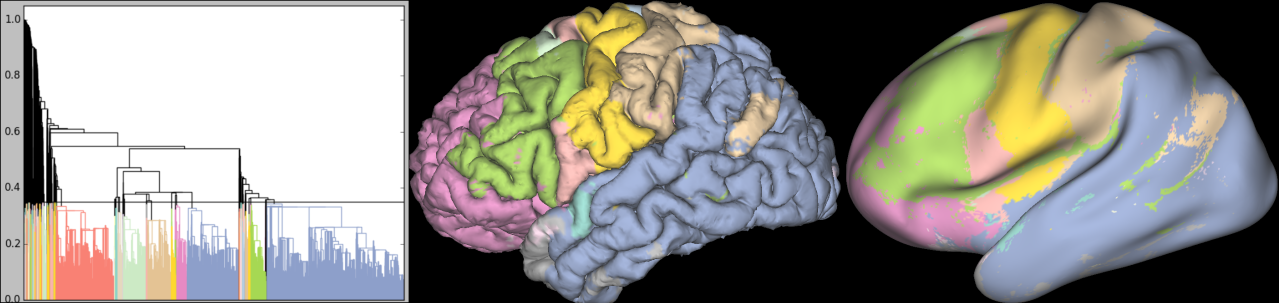
\includegraphics[width=\textwidth]{img/all_brain/moreno_10000.png}
    \caption{Parcelamiento de la corteza utilizando el m\'etodo de 
             Moreno-Dominguez. Las primeras $10000$ uniones fueron entre
             $clusters$ vecinos.}
    \label{fig:moreno_corteza0}
\end{figure}

\begin{figure}[h!]
    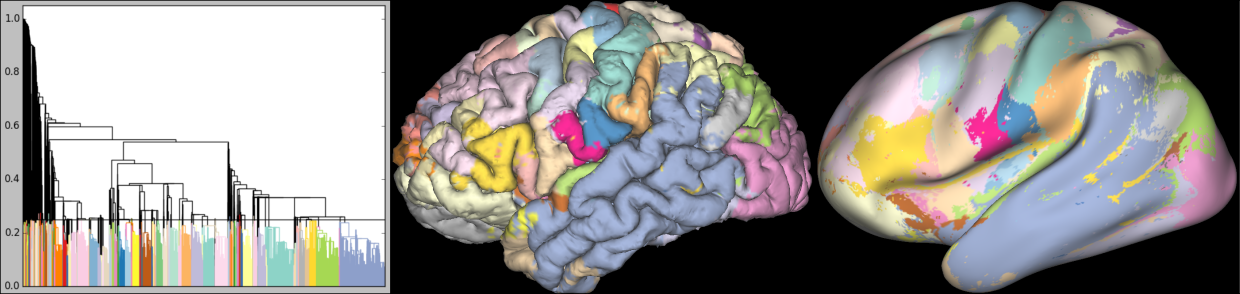
\includegraphics[width=\textwidth]{img/all_brain/moreno_10000_deep0.png}
    \caption{Parcelamiento de la corteza utilizando el m\'etodo de 
             Moreno-Dominguez. Las primeras $10000$ uniones fueron entre
             $clusters$ vecinos. Corte con mayor profundidad en el 
             dendrograma.}
    \label{fig:moreno_corteza1}
\end{figure}

\begin{figure}[h!]
    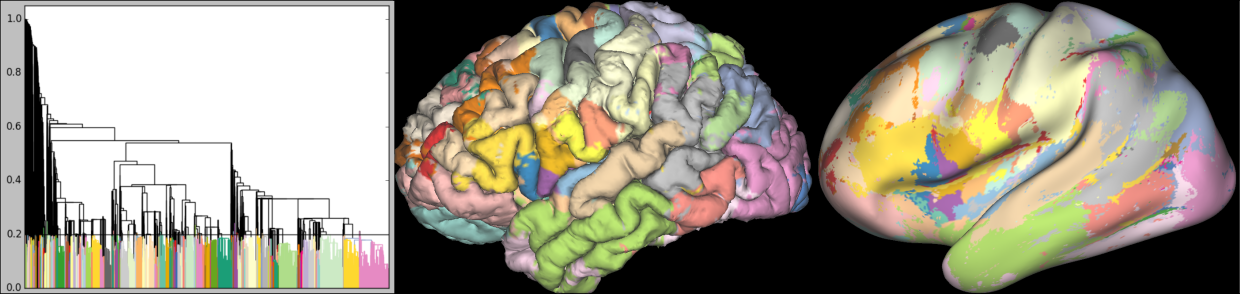
\includegraphics[width=\textwidth]{img/all_brain/moreno_10000_deep1.png}
    \caption{Parcelamiento de la corteza utilizando el m\'etodo de 
             Moreno-Dominguez. Las primeras $10000$ uniones fueron entre
             $clusters$ vecinos. Corte con a\'un mayor profundidad en el 
             dendrograma.}
    \label{fig:moreno_corteza2}             
\end{figure}

\subsection{Utilizando nuestro m\'etodo}
\label{sec:corteza_nuestro}

Por \'ultimo parcelamos el hemisferio usando el m\'etodo de 
Moreno-Dominguez. Al igual que en la secci\'on \label{ch:nuestro},
descartamos los tractogramas con un solo voxel visitado y aplicamos un
$threshold$ de $0.25$ en cada voxels. Las figuras 
\ref{fig:nosotros_corteza0} y \ref{fig:nosotros_corteza1} muestran 
las parcelas obtenidas sin aplicar restricciones en ninguna iteraci\'on
del $clustering$ ($k=0$). Ambas muestran el resultado obtenido de un mismo
dendrograma cortado a distintos niveles de profundidad. Las figuras 
\ref{fig:nosotros_corteza2}; \ref{fig:nosotros_corteza3} y
\ref{fig:nosotros_corteza4} muestran los resultados usando $k=20000$ a
distintos niveles de profundidad del dendrograma. Esto es, las primeras
$10000$ uniones son solo entre $clusters$ vecinos y de tama\~no 
homog\'eneo. 

\begin{figure}[h!]
    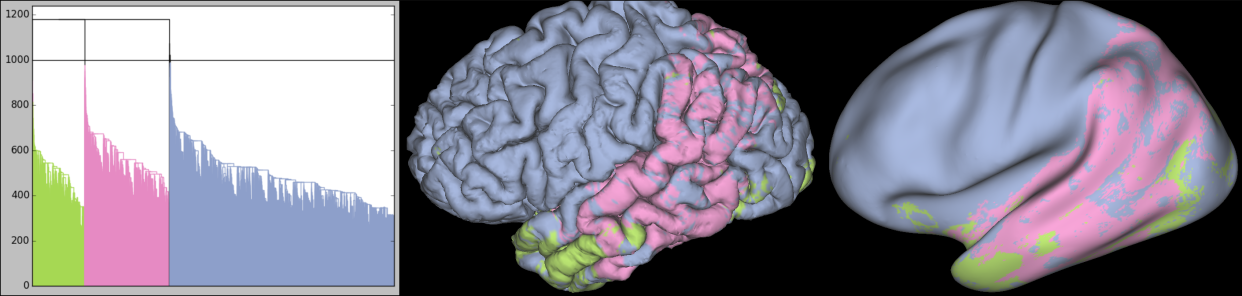
\includegraphics[width=\textwidth]{img/all_brain/logit_0.png}
    \caption{Parcelamiento de la corteza utilizando nuestro m\'etodo
             sin aplicar restricciones en ninguna iteraci\'on.}
    \label{fig:nosotros_corteza0}
\end{figure}
                                                                                                                        
\begin{figure}[h!]
    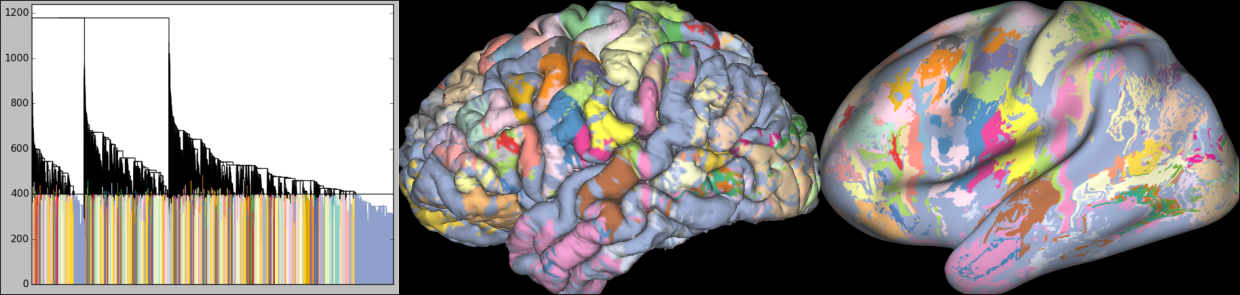
\includegraphics[width=\textwidth]{img/all_brain/logit_0_deep.png}
    \caption{Parcelamiento de la corteza utilizando nuestro m\'etodo
             sin aplicar restricciones en ninguna iteraci\'on. Corte con
             mayor profundidad en el dendrograma.}
    \label{fig:nosotros_corteza1}
\end{figure}

\begin{figure}[h!]
    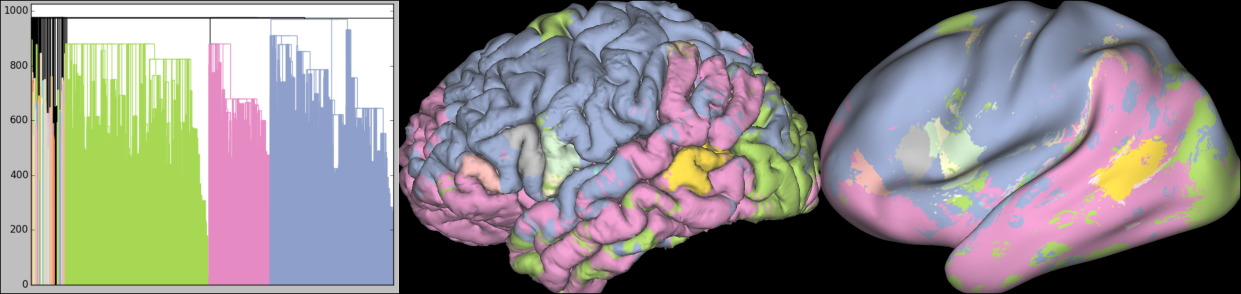
\includegraphics[width=\textwidth]{img/all_brain/logit_20000.png}
    \caption{Parcelamiento del \'area de Broca utilizando nuestro m\'etodo.
             Las primeras $20000$ uniones fueron entre $clusters$
             vecinos.}    
    \label{fig:nosotros_corteza2}
\end{figure}

\begin{figure}[h!]
    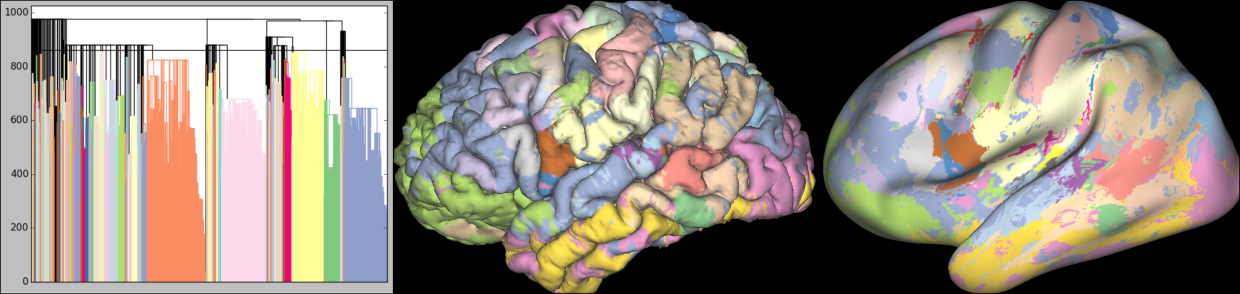
\includegraphics[width=\textwidth]{img/all_brain/logit_20000_deep0.png}
    \caption{Parcelamiento del \'area de Broca utilizando nuestro m\'etodo.
             Las primeras $20000$ uniones fueron entre $clusters$
             vecinos. Corte con mayor profundidad en el dendrograma. }    
    \label{fig:nosotros_corteza3}
\end{figure}

\begin{figure}[h!]
    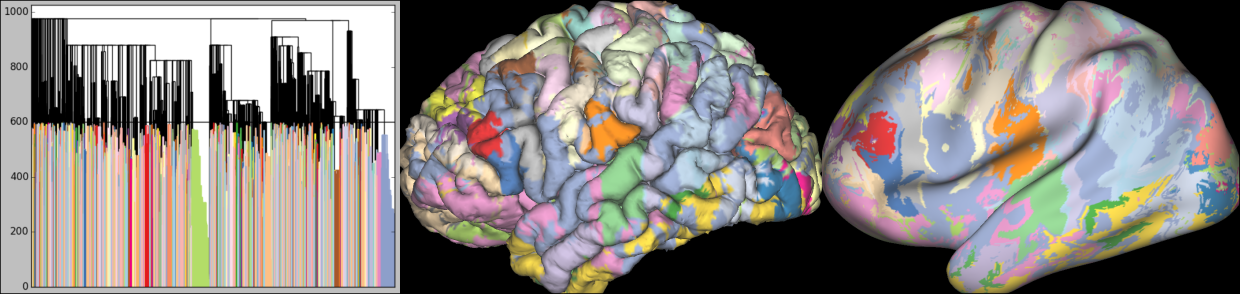
\includegraphics[width=\textwidth]{img/all_brain/logit_20000_deep1.png}
    \caption{Parcelamiento del \'area de Broca utilizando nuestro m\'etodo.
             Las primeras $20000$ uniones fueron entre $clusters$
             vecinos. Corte con a\'un mayor profundidad en el
             dendrograma. }    
    \label{fig:nosotros_corteza4}
\end{figure}

\subsection{Resultados de los m\'etodos en mayor detalle}
\label{sec:acercamiento_corteza}

A diferencia de lo que suced\'ia con el \'area de Broca, es dif\'icil
comparar
los resultados visualmente. Sin embargo presentamos dos parcelaciones
obtenidas para que puedan ser observadas en mayor detalle. La figura 
\ref{fig:vs_moreno} presenta la corteza parcelada usando el m\'etodo 
Moreno-Dominguez con $k=10000$. Esto es, las primeras $10000$ uniones
son solo entre $clusters$ vecinos y de tama\~no homog\'eneo. La figura 
\ref{fig:vs_nosotros} muestra el resultado de usar nuestro m\'etodo con
$k=20000$.

\begin{figure}[h!]
    \centering
    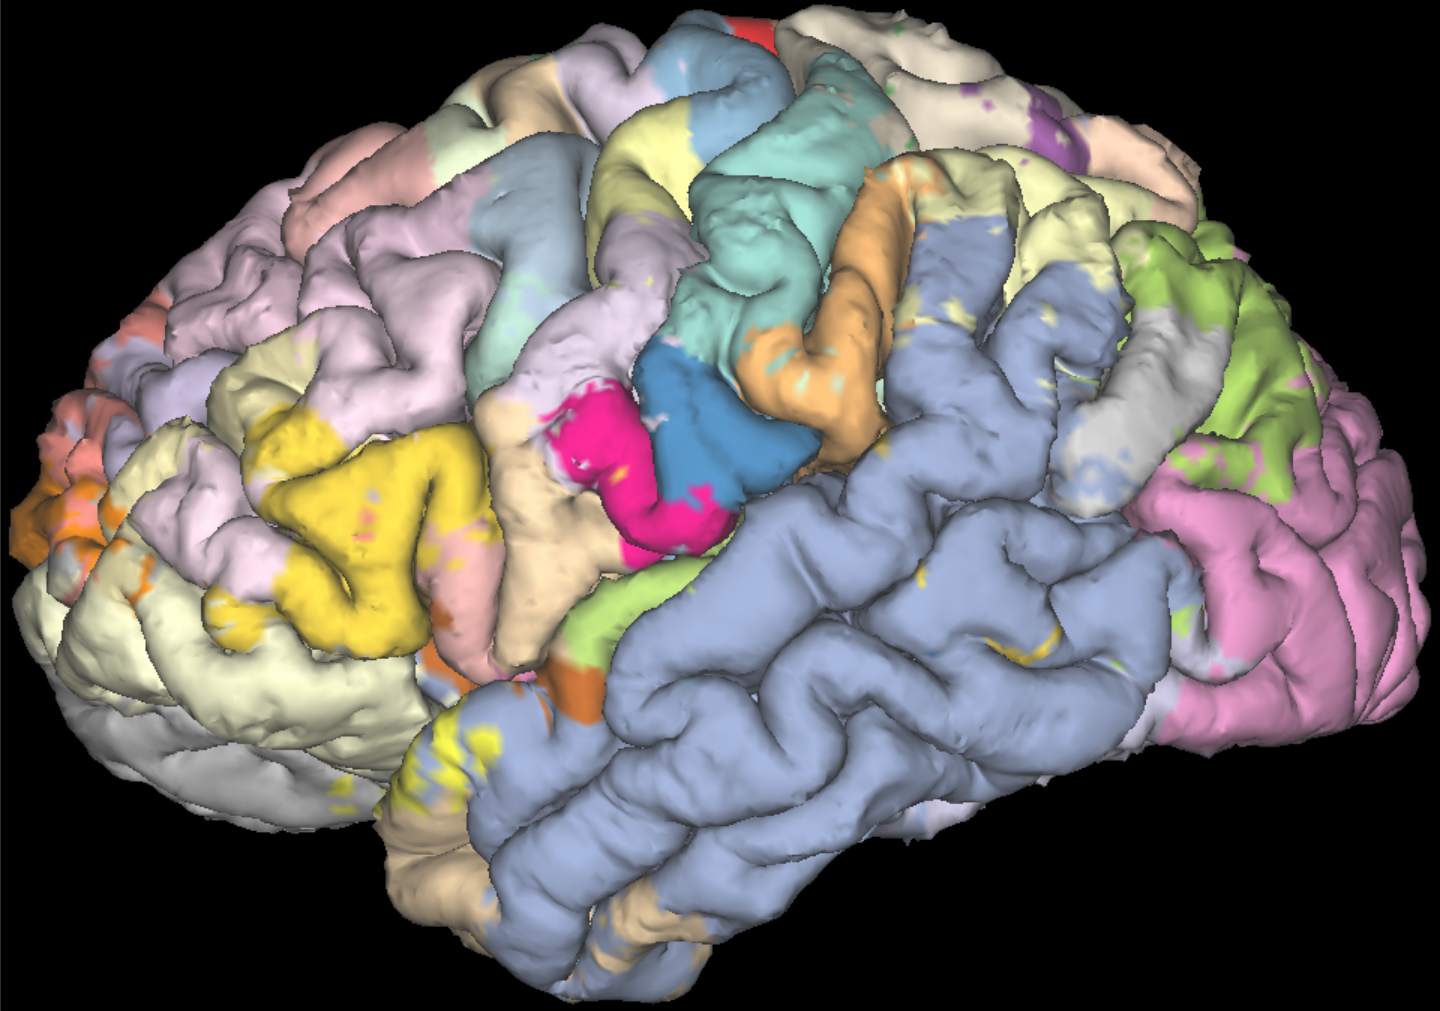
\includegraphics[width=0.7\textwidth]{img/all_brain/vs_moreno.png}
    \caption{Detalle sobre las parcelas obtenidos utilizando 
             el m\'etodo de Moreno-Dominguez. Las primeras $20000$
             uniones fueron entre $clusters$ vecinos. }    
    \label{fig:vs_moreno}
\end{figure}

\begin{figure}[h!]
    \centering
    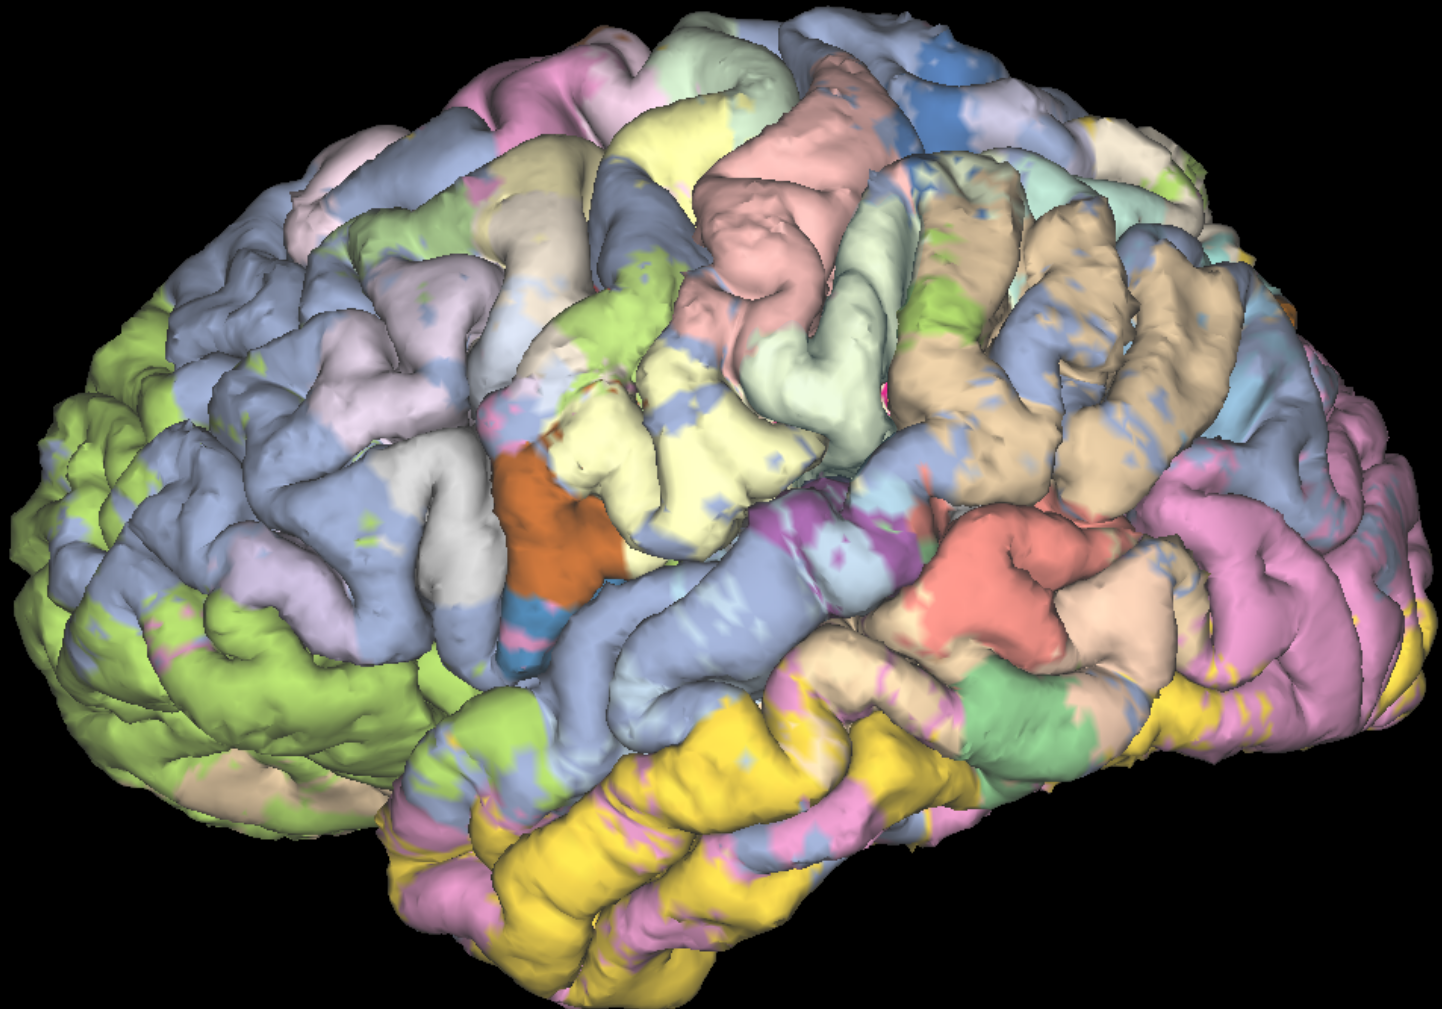
\includegraphics[width=0.7\textwidth]{img/all_brain/vs_nuestro.png}
    \caption{Detalle sobre las parcelas obtenidos utilizando 
             nuestro m\'etodo. Las primeras $20000$
             uniones fueron entre $clusters$ vecinos. }    
    \label{fig:vs_nosotros}
\end{figure}


